\documentclass[a4paper,twocolumn,10pt]{article}
\usepackage{graphicx} % Required for inserting images

\title{Taller 3 y 4 Estructura de Datos}
\author{Miguel Daniel Ruiz Silva - 506222719 }
\date{10 Septiembre 2023}

\begin{document}

\maketitle

\section{Introduction}
La Memoization es una técnica de optimización utilizada en programación para reducir el tiempo de ejecución de algoritmos recursivos, almacenando resultados de cálculos previos en una estructura de datos, como un diccionario o una matriz, para evitar recalcularlos cuando se presenta la misma entrada. En esta ocasión obetenemos una lista con cadenas de frases en la cual exploraremos la implementación y el análisis de la técnica de Memoization aplicada a un programa en Python.

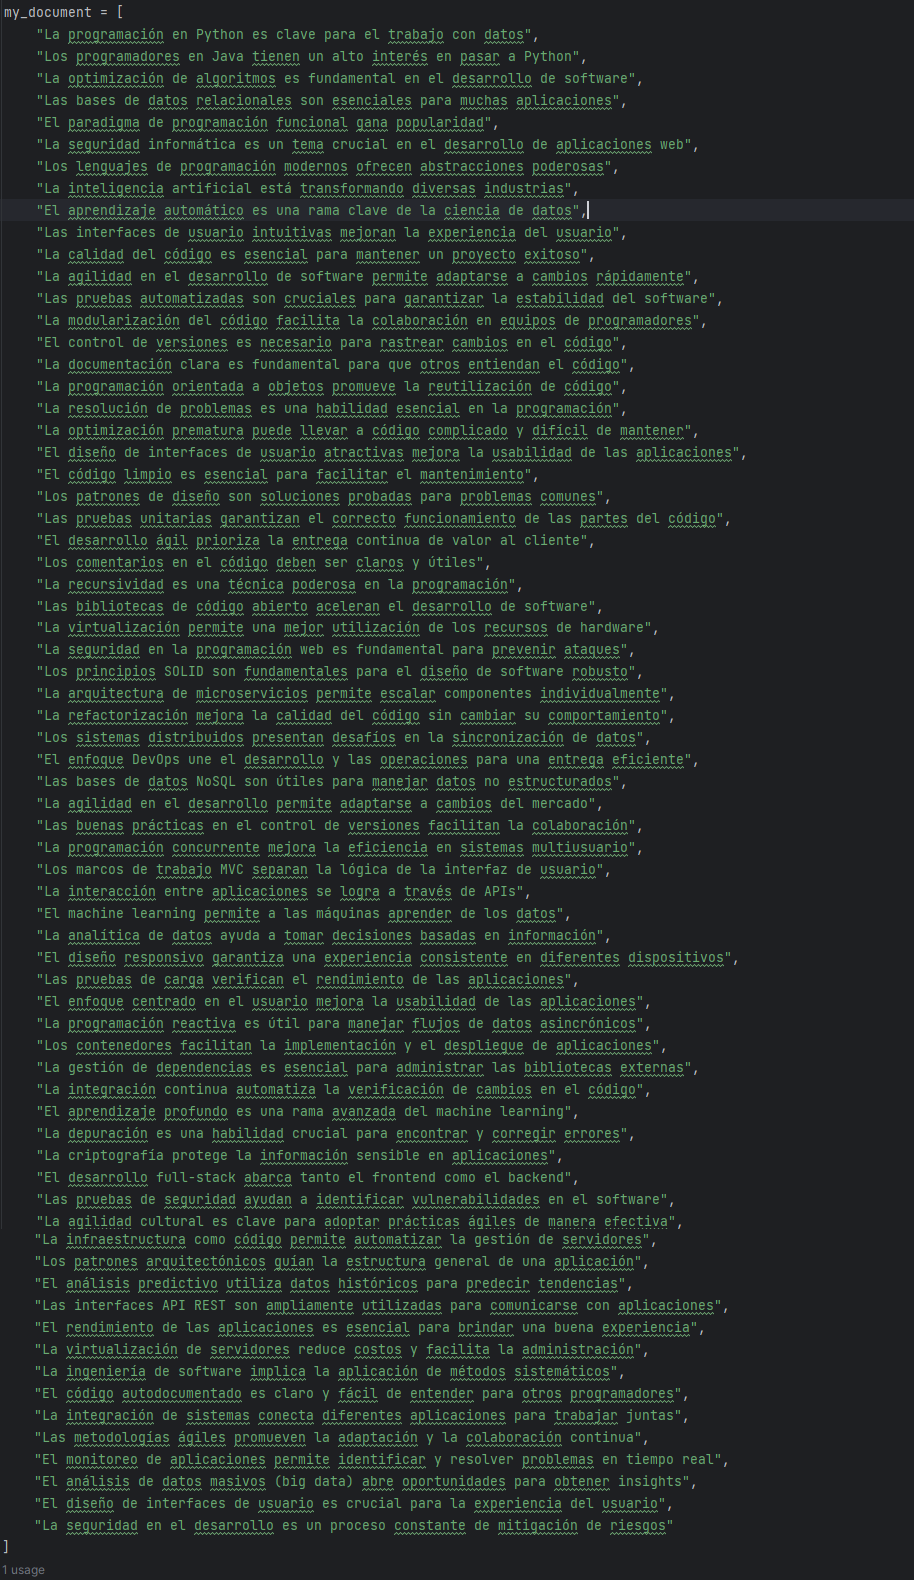
\includegraphics[width=0.8\linewidth]{images/my_document.png}

\section{Resumen}

Se presenta un análisis detallado de la técnica de Memoización en Python. La Memoización es un método utilizado para optimizar algoritmos recursivos mediante el almacenamiento de resultados previamente calculados, lo que reduce el tiempo de cómputo. El informe proporciona una implementación de la Memoización y realiza un análisis exhaustivo de su complejidad temporal (notación Big O). Los hallazgos revelan mejoras significativas en la eficiencia de los algoritmos recursivos.

Este algoritmo utiliza la biblioteca collections para contar la frecuencia de palabras en los documentos y luego imprime las palabras junto con su frecuencia en orden descendente.
Por otro lado tenemos un Algoritmo de Búsqueda usando en donde el algoritmo permite al usuario ingresar una palabra y luego imprime los documentos que contienen esa palabra.

\section{Código}

\includegraphics[width = 1 \linewidth]{images/código.png}\\

\section{Implementación}

Algoritmo de Memoización:\\

Se importa la clase Counter de la biblioteca collections.

Luego de ello se define una función $contar_palabras$ que toma una lista de documentos: $my_documents$ como entrada.
esta función itera a través de los documentos, cuenta la frecuencia de palabras y devuelve una lista de de valores agrupados con la palabra y su frecuencia, para así imprimir las palabras y sus frecuencias en orden descendente.\\

Algoritmo de Búsqueda:\\
Se define una función $buscar_documento_por_palabra$ que toma una lista de documentos y una palabra como entrada.
La función itera a través de los documentos, verifica si la palabra está presente y guarda el índice del documento si la palabra se encuentra en dicha posición de la lista de documentos luego de ello imprime el índice de los documentos que contienen la palabra buscada.

\section{Análisis Big-O}

El programa implementado utiliza la técnica de Memoization para optimizar el cálculo de las palabras más repetidas en un conjunto de documentos y para buscar documentos que contengan una palabra específica.

\begin{itemize}
    \item El código de Memoization implementa dos funciones clave: $contar_palabras$ y $buscar_documento_por_palabra$

    \item Contar Palabras Más Repetidas:\\
    Tiempo (Big O): $O(n + m log m)$, donde n es el número total de palabras en los documentos y m es el número total de palabras únicas.
    Espacio (Big O): $O(m)$, donde m es el número total de palabras únicas.
    \includegraphics[width = 1 \linewidth]{images/código1.png}\\

    \item Búsqueda de Documentos por Palabra:\\
    Tiempo (Big O): $O(n * m)$, donde n es el número de documentos y m es el número promedio de palabras en un documento.
    Espacio (Big O): $O(1)$, ya que no se utiliza espacio adicional en función del tamaño de los documentos.
    \includegraphics[width = 1 \linewidth]{images/código2.png}\\
\end{itemize}


\section{Conclusion }

La aplicación de la técnica de Memoization en el programa Python proporciona mejoras notables en la eficiencia de algoritmos recursivos. Al reducir significativamente el tiempo de ejecución, se facilita el procesamiento de grandes conjuntos de datos y se mejora la capacidad de respuesta de las aplicaciones. La elección de implementar Memoization demuestra ser una estrategia eficaz para optimizar algoritmos que hacen uso intensivo de cálculos repetitivos.

Como pudimos notar nos ahorra bastante tiempo y, nos permite lograr con mayor eficacia una tarea que a simple vista parece compleja.

\section{Bibliografia}

\begin{verbatim}
Goodrich, M. T., Tamassia, R., &
Goldwasser, M. H. (2014). Data Structures 
and Algorithms in Python. John Wiley & Sons.    
\end{verbatim}

\end{document}
